\chapter{User Manual}

\section{Admin}
\begin{figure}
\centering
	\frame{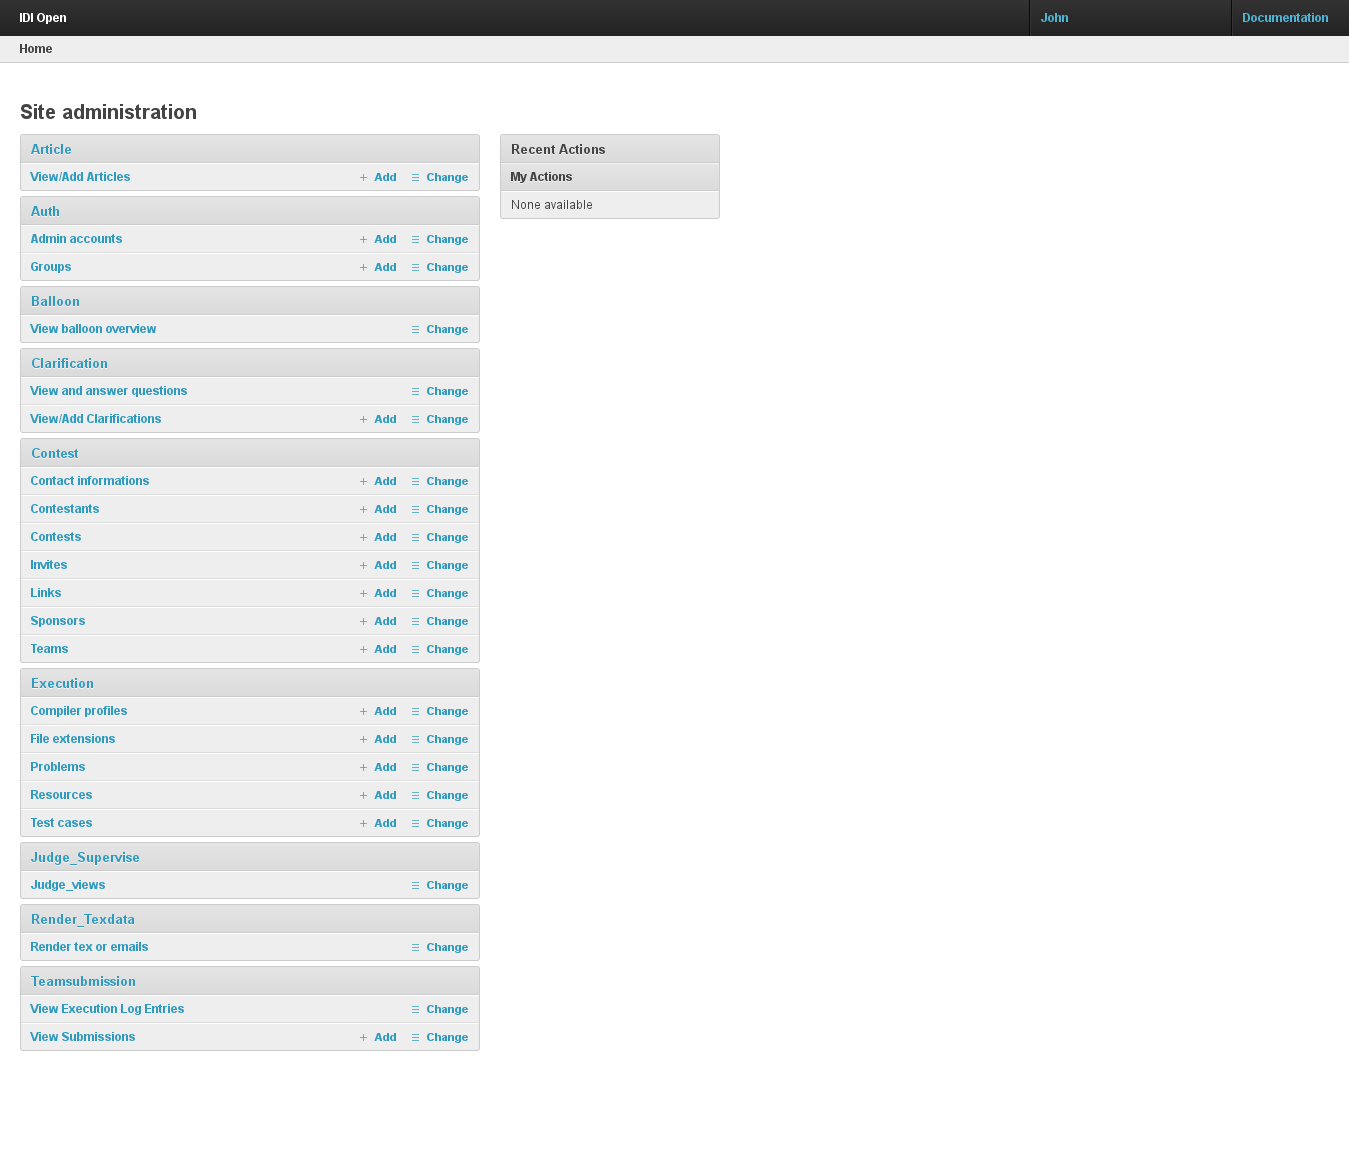
\includegraphics[width=0.8\textwidth]{Usermanual-img1.png}}
	\caption{Admin overview}
	\label{fig:adminOverview}
\end{figure}

In Fig~\ref{fig:adminOverview} you can see how the admin page looks. Here you will find
most of the tools to successfully host a competition. This part of the
user manual will contain information around the admin interface, and
how to use it. The admin interface is a tool for creating, editing and
deleting objects, objects in this sense is basicly database entries.
When referring to objects later, this is what we mean by that.


\subsection{Basic Usage}

\subsubsection{Creating Objects}

To create a new object simply select what kind of object you would like
to create, and click the add button next to its name. This button is
shown in Figure~\ref{fig:createContest}, and the list of available objects can be seen in
on the front page of the admin interface(Figure~\ref{fig:adminOverview}).

\subsubsection{Editing Objects}
\label{sec:editObjects}

To edit existing objects you first have to locate the object you wish to
edit. This is done by selecting the type you want in the main menu.
This will open a list display of all objects in that category. If the
list allows it, you can apply filters and search for the object you
would like to edit. When you have found this object, simply click it
and a editing form will appear. Make your changes and click the save
button.

\subsubsection{Deleting Objects}

When deleting objects you open the list display as explained in the
previous section(~\ref{sec:editObjects}), select the item(s) you would like to delete,
and select the delete action in the lower left corner. This will open a
confirmation view, displaying any related objects that will cascade if
you wish to continue. The edit form also includes a delete button.



\subsection{Creating a Contest}

To create a contest, first navigate to the contest part of the admin
menu, and click the Add link next to Contests (Figure~\ref{fig:createContest})

\begin{figure}
\centering
	\frame{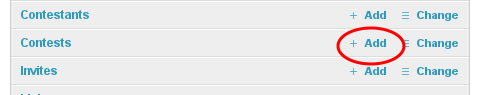
\includegraphics[width=0.8\textwidth]{Usermanual-img2.png}} 
	\caption{Create contest}
	\label{fig:createContest}
\end{figure}

Fill in the given form with the data relevant for your contest. If this
is your first contest or a fresh system, you will also have to create
contact information and links for the navigation.

\begin{figure}
\centering
	\frame{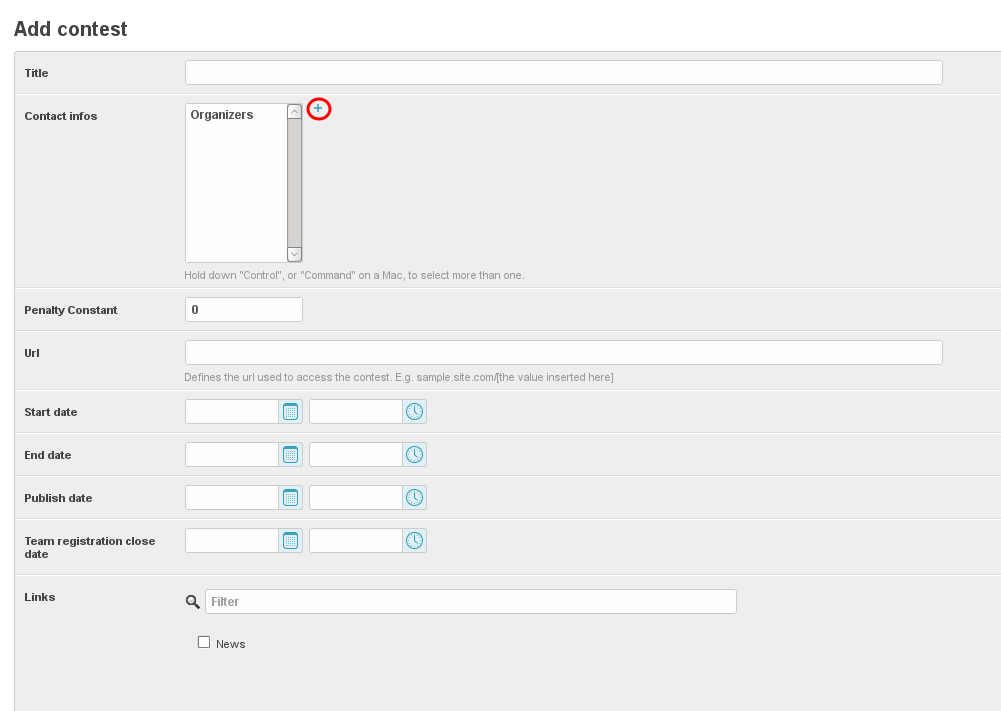
\includegraphics[width=0.8\textwidth]{Usermanual-img3.png}} 
	\caption{Contest create form}
	\label{fig:contestCreateForm}
\end{figure}

To create new contact information, click the plus sign as highlighted in
Figure~\ref{fig:contestCreateForm}. The same applies for Links and Sponsors. The Penalty
Constant is a variable used to calculate the score for each team. This
value is a penalty in minutes for each wrong solution submitted. The
Url field is a unique variable for each contest that sets the url
location for the contest. E.g if the url variable is
{\textquotedblleft}test{\textquotedblright} then the contest will be
located at \textit{http://example.com/test/}. 

The next four fields are time and data objects that determine when the
contests is starting, ending, when it should be published, and when the
registration should close.

\subsubsection{Create Links}

To create a link, click the plus sign in the links section like
explained above for contact information. This will open a pop-up window
as shown in Figure~\ref{fig:createLink}.

\begin{figure}
\centering
	\frame{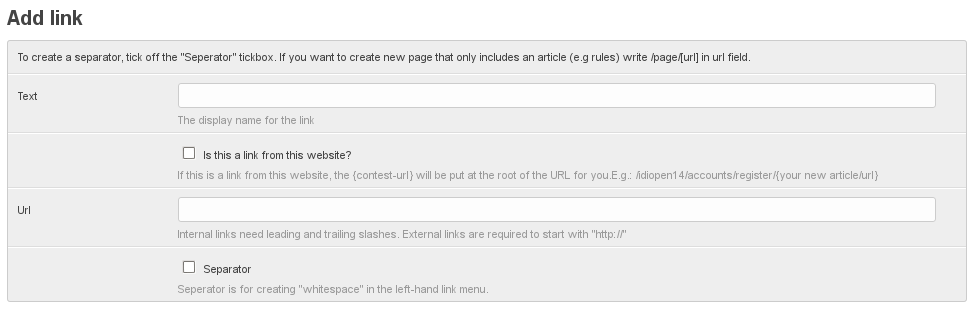
\includegraphics[width=0.8\textwidth]{Usermanual-img4.png}} 
	\caption{Create link}
	\label{fig:createLink}
\end{figure}

These links will show up in the main navigation in the contest page. The
text field will be the displayed text and the url will be the target
url for the link. If this is an internal link to somewhere on the
contest page, then select the checkbox indicating that. This will cause
the contest url being appended before the defined url. You can also
create a separator by checking the separator checkbox. This will create
a separated field in the navigation, allowing you to group relevant
links together.

It is also possible to sort the link by drag and drop to achieve the
sorting you want. And to add or remove an existing link, you just have
to check or uncheck the checkbox. These features are depicted in Figure~\ref{fig:linkSelectOrder}.

\begin{figure}
\centering
	\frame{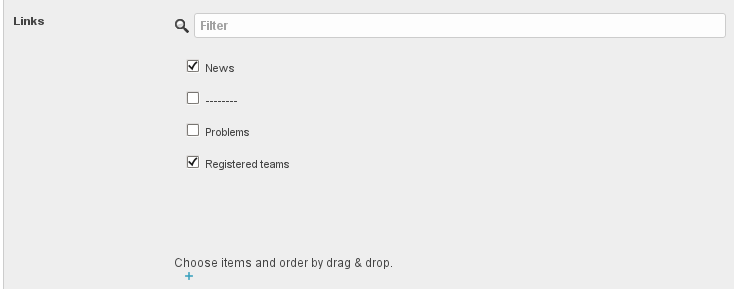
\includegraphics[width=0.8\textwidth]{Usermanual-img5.png}} 
	\caption{Links selection and ordering}
	\label{fig:linkSelectOrder}
\end{figure}

\subsubsection{Create Sponsor}

To create a sponsor you click the plus icon in the sponsor section. This
will open up a pop-up similar to the Links creation. 

\begin{figure}
\centering
 	\frame{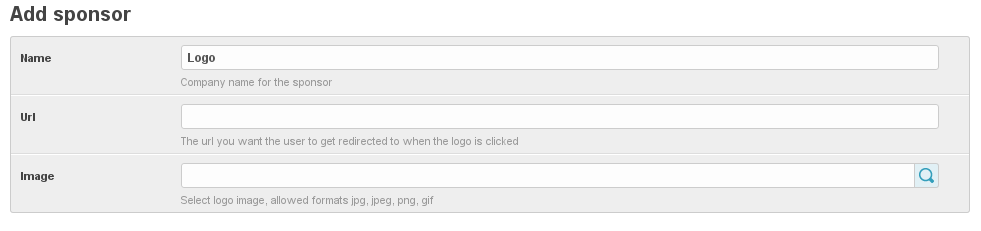
\includegraphics[width=0.8\textwidth]{Usermanual-img6.png}} 
 	\caption{Create sponsor}
 	\label{fig:createSponsor}
\end{figure}

to link to, and click the magnifying glass to browse and upload images.
This will open up the file browser in another pop-up window as you can
see in Figure~\ref{fig:sponsorUpload}. To upload a new image, click the Upload button in
the top right corner. Upload your image and click Sponsor in the top
left navigation to go back to the files. The system automatically
scales images down to appropriate sizes. For sponsor images you should
use Small images as shown in Figure~\ref{fig:sponsorUpload}. 

\begin{figure}
\centering
	\frame{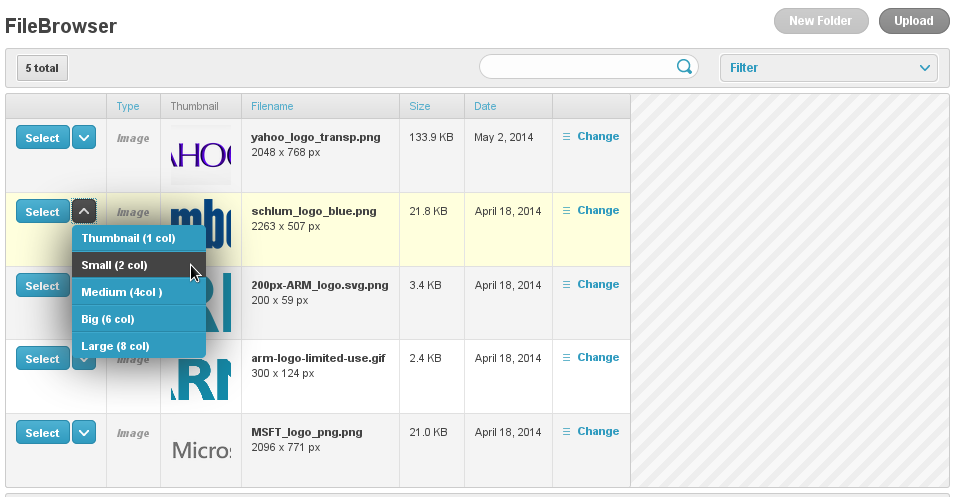
\includegraphics[width=0.8\textwidth]{Usermanual-img7.png}} 
 	\caption{Sponsor select and image upload}
 	\label{fig:sponsorUpload}
\end{figure}


\subsubsection{Create Compiler Profile}

A compiler profile is a object with specifications on how a programming
language should be compiled and executed. Each compiler profile
includes a list of file extensions that should be allowed. These are
added the same way as previously explained(By clicking the plus sign).

The compile and run fields both take a string of text used to compile
and run the submission. The filename and basename will be inserted in
the string where the tags \{BASENAME\} and \{FILENAME\} are present.

\begin{figure}
\centering
	\frame{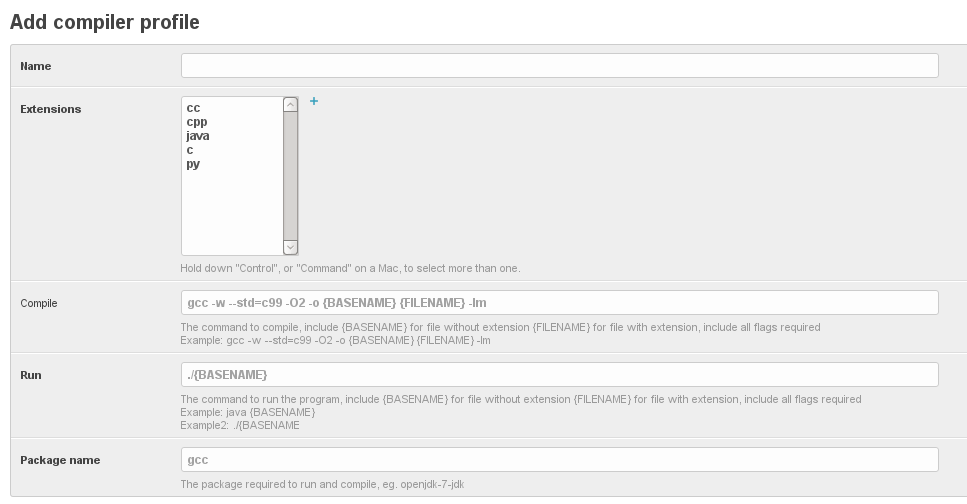
\includegraphics[width=0.8\textwidth]{Usermanual-img8.png}} 
	\caption{Compiler profile}
	\label{fig:compilerProfile}
\end{figure}



\bigskip

\subsubsection{Create Problems}

Problems are the tasks that contestants will solve when the contest
starts. The problem form includes a problem title, description with
WYSIWYG editor support, and a text file. Each problem is also linked to
a single contest. For each problem you also need test cases, and a set
of resource limits for the different compiler profiles. These models
will be explained in the next sections.


\begin{figure}
\centering
	\frame{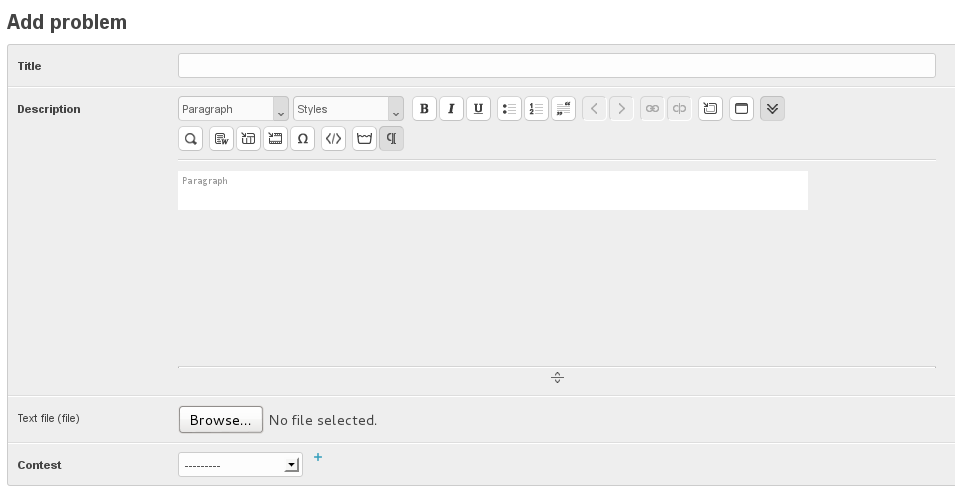
\includegraphics[width=0.8\textwidth]{Usermanual-img9.png}} 
	\caption{Create problem}
	\label{fig:problem}
\end{figure}

\subsubsection{Create Test Case}

Each test case is linked to a problem, and there can be multiple test
cases per problem. The most important parts of the test case is the
input and output files. The input file will get parsed by the
submissions, and the output file matched against the submission output.
The test case also includes a short description and a description of
the input and output. A screenshot of the test case creation can be
seen in Figure~\ref{fig:problem}. 


\bigskip

If the problem uses floating points or in any other way cannot be
matched to a single output file, then you can set the test case to use
a custom validator. This is a program that takes the output from the
submission and the output file specified as input. The output from the
validator should be 1 for correct answer and 0 for wrong answer. \ 

\begin{figure}
\centering
	\frame{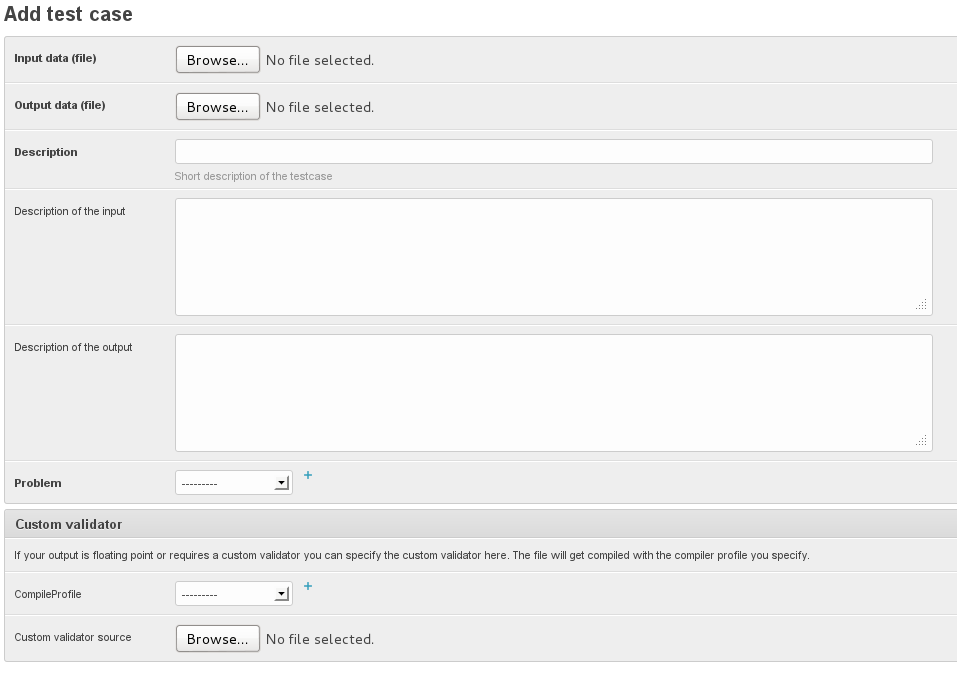
\includegraphics[width=0.8\textwidth]{Usermanual-img10.png}} 
	\caption{Test case}
	\label{fig:testCase}
\end{figure}


\subsubsection{Resource}

Each problem requires a set of resource limitations for the different
compiler profiles. THese limits sets the amount of resources the
uploaded program is allowed to use, and if they exceed that amount they
submission will be marked as a wrong answer. As shown in Figure~\ref{fig:resource},
the different fields are, max compile time, max program timeout, max
memory, max processes, and max filesize. The resources depend on the
problem and the programming language. C is a language that runs very
fast and effective, and java requires a huge amount of memory to boot
the Java Virtual Machine. So it can be quite difficult to set precise
limits. It is also possible to give unlimited amounts by setting -1 as
the value.


\begin{figure}
\centering
	\frame{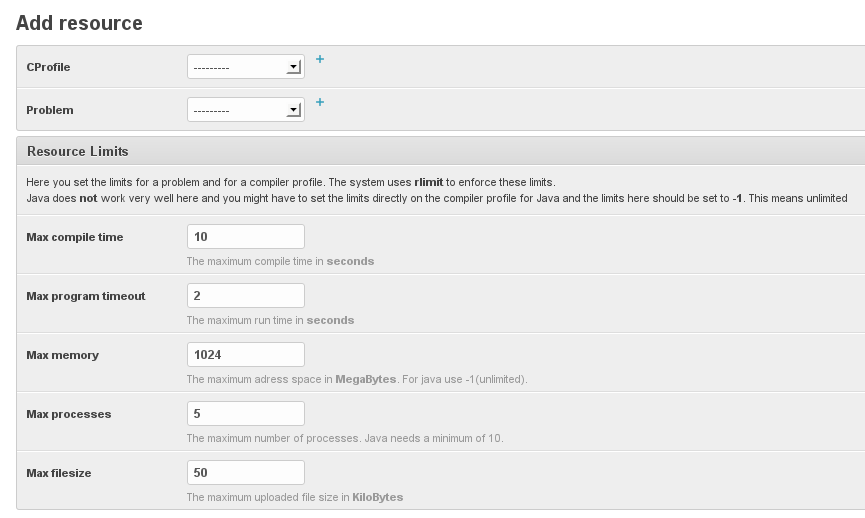
\includegraphics[width=0.8\textwidth]{Usermanual-img11.png}} 
	\caption{Resource}
	\label{fig:resource}
\end{figure}

\subsection{Creating Articles}

Articles is the main way of communicating with users of the system. The
most recent and important news are placed on the front page. Other news
can be found in the article list.

Articles consists mainly of a title and a body. The other fields are
optional and configures how and where the article should be displayed.
The text is written in a WYSIWYG editor and is integrated with the file
browser described earlier. This gives the opportunity to make formatted
news which can be easily edited again later. Article is also used for
creating content that should not be considered as news. E.g. rules,
history, FAQ. If this is wanted you can uncheck the Visible Article
List checkbox. You also have the ability to create custom links for
articles that should be available as an url. Articles can also be
marked as urgent, what this means is that they will reside on the top
of the frontpage and article list.

\begin{figure}
\centering
	\frame{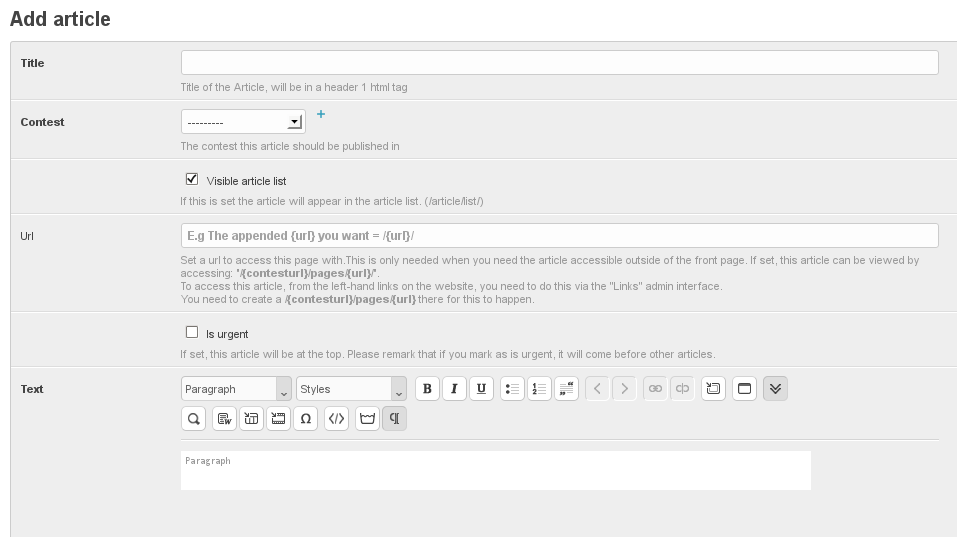
\includegraphics[width=0.8\textwidth]{Usermanual-img12.png}} 
	\caption{Add article}
	\label{fig:article}
\end{figure}

\subsection{Create User}

\subsubsection{Create Contestant}

If a user is unable to create a user on their own, or if you wish to
create it through the admin interface. Click the add button next to
contestants in the main menu. This will bring up the form shown in
Figure~\ref{fig:createContestant}. Simply fill in the information you want.

\begin{figure}
\centering
	\frame{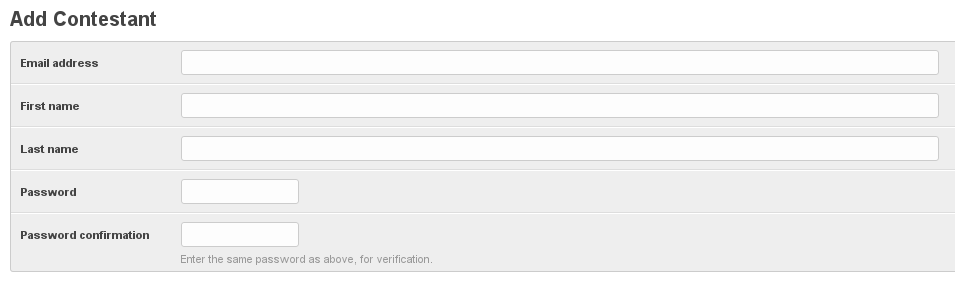
\includegraphics[width=0.8\textwidth]{Usermanual-img13.png}} 
	\caption{Create contestant}
	\label{fig:createContestant}
\end{figure}


\subsubsection{Create Admin User}

To create an admin user the process i very similar to create a
contestant. You click the add button next to Admin accounts in the main
menu. This will bring up a more detailed form than the contestant form,
and is shown in Figure~\ref{fig:createAdmin}. This form as the extra fields Active,
Staff status, and superuser status. The staff status sets whether the
user should have access to the admin panel, and Superuser status gives
the user all permissions. This form also includes a tools for setting
group permissions and individual permissions. 

\begin{figure}
\centering
	\frame{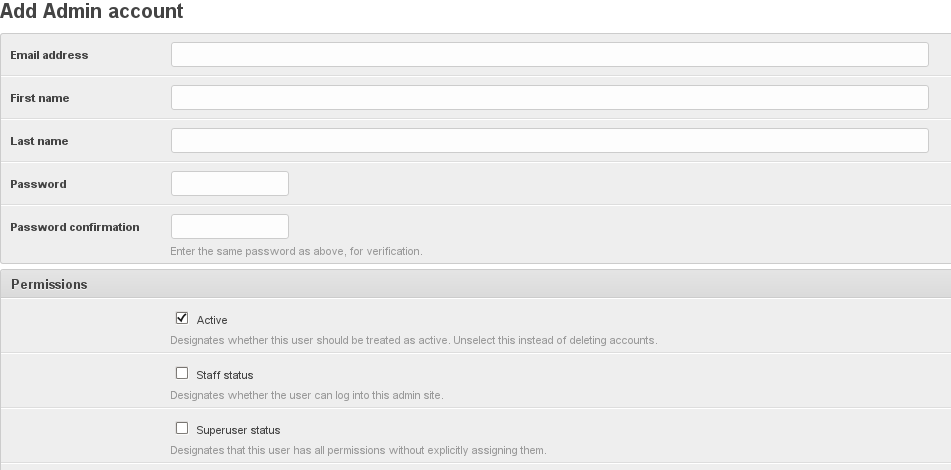
\includegraphics[width=0.8\textwidth]{Usermanual-img14.png}} 
	\caption{Admin account}
	\label{fig:createAdmin}
\end{figure}

\subsubsection{Promote Contestant to Admin}

If you would like to promote a regular user to a staff user, then all
you have to do is edit the the user in question, and check the Staff
status checkbox as shown in Figure~\ref{fig:promoteUser}. The user will now be removed
from the Contestant view, and moved to the Admin accounts view. 

\begin{figure}
\centering
	\frame{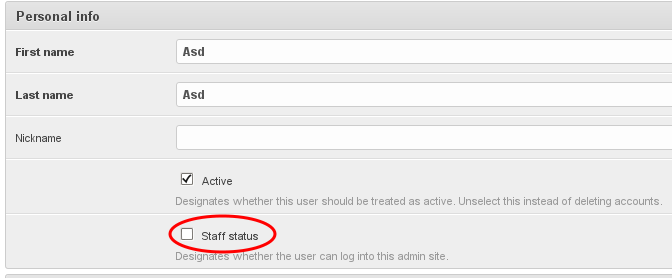
\includegraphics[width=0.8\textwidth]{Usermanual-img15.png}} 
	\caption{Promote user}
	\label{fig:promoteUser}
\end{figure}


\subsection{Balloon View}

The balloon view covers the functionality meant for balloon
functionaries. Clicking on View Balloon Overview, located in the
section Balloon, will take you to the balloon view. 

\begin{figure}
\centering
	\frame{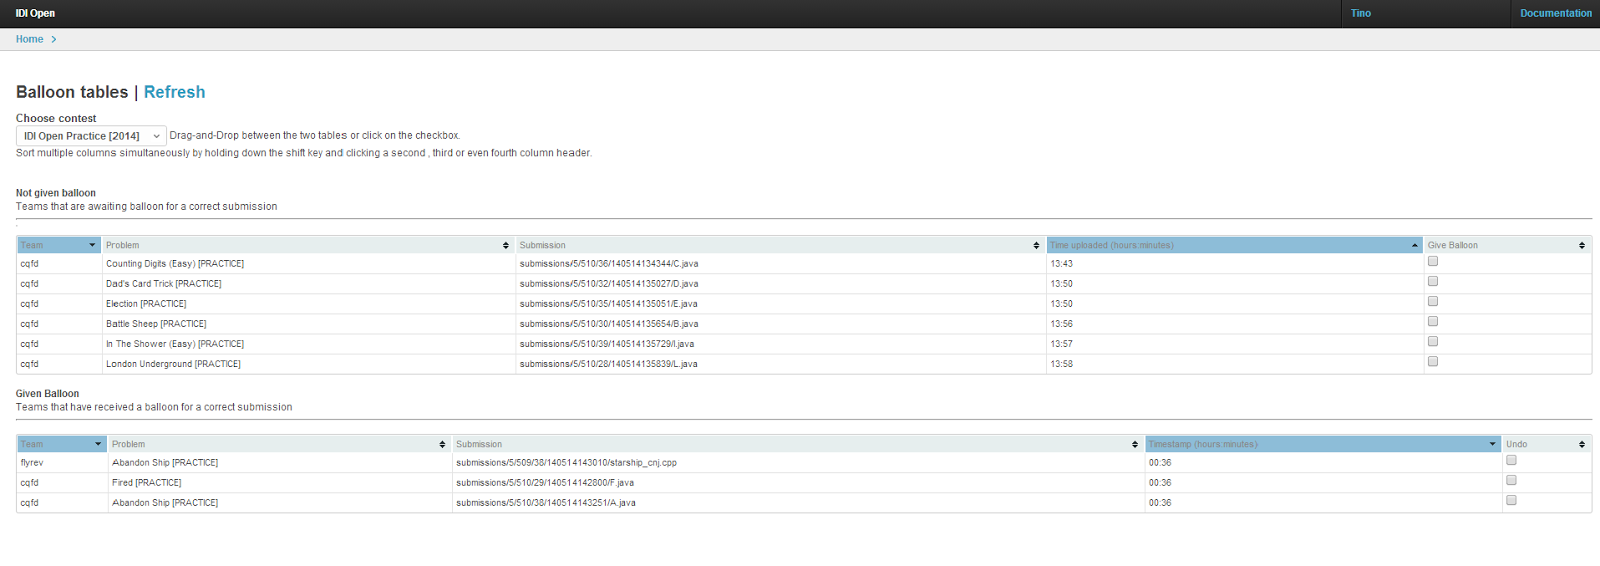
\includegraphics[width=0.8\textwidth]{Usermanual-img16.png}} 
	\caption{Balloon view}
	\label{fig:balloonView}
\end{figure}

The first choice you are met with, is which contest you want to show
submissions from. The drop down menu lets you pick any of the already
created contests. The balloon view consists of two tables. The first
table is named, not given balloon, and contains the onsite teams that
are awaiting a balloon for a correct submission. The table consists of
five columns covering the essential information a balloon functionary
needs to know. The table is automatically sorted on team and time
uploaded, but this can be changed by the user. All the columns in the
table are sortable.

The rightmost column consists of checkboxes for each row in the table.
We have given the balloon functionaries two different possibilities to
register that a team has been given a balloon. The balloon functionary
can either press the corresponding checkbox for the team, in the
rightmost column, or drag the respective row to the table beneath. This
will move the row from the first table, to the second table.

The second table is named, Given Balloon, and contains teams that have
received a balloon for a correct submission. This table has the same
functionality as the first table. The rightmost column, Undo, consists
of checkboxes. If you press a checkbox, or drag the row to the other
table, it will cause the row to change tables. This gives the balloon
functionaries total control, in case of a misclick.


The last function the balloon table has is that it will tell you when
new submissions has arrived. The blue
{\textquotedblleft}Refresh{\textquotedblright} text located at the top
left corner, will change to {\textquotedblleft}New
submission{\textquotedblright}, when a new submission arrives. Pressing
the text will refresh the page, and new submissions will show up in the
first table, not given balloon. 


\subsection{Judge View}

In the section called Judge\_Supervise there{\textquoteright}s a link
labeled Judge\_views. This takes you to the site primarily intended for
inspecting the submissions in the system. 

This is the starting point for staff users wanting to inspect a
submission. Starting at the top there{\textquoteright}s a drop down
menu enabling you to inspect submissions for a specific contest,
labeled {\textquotedblleft}Choose contest{\textquotedblright}. Further
down there{\textquoteright}s another drop down menu enabling you to
take a closer look at a single team, we will take a closer look at this
in the next section. 

\begin{figure}
\centering
	\frame{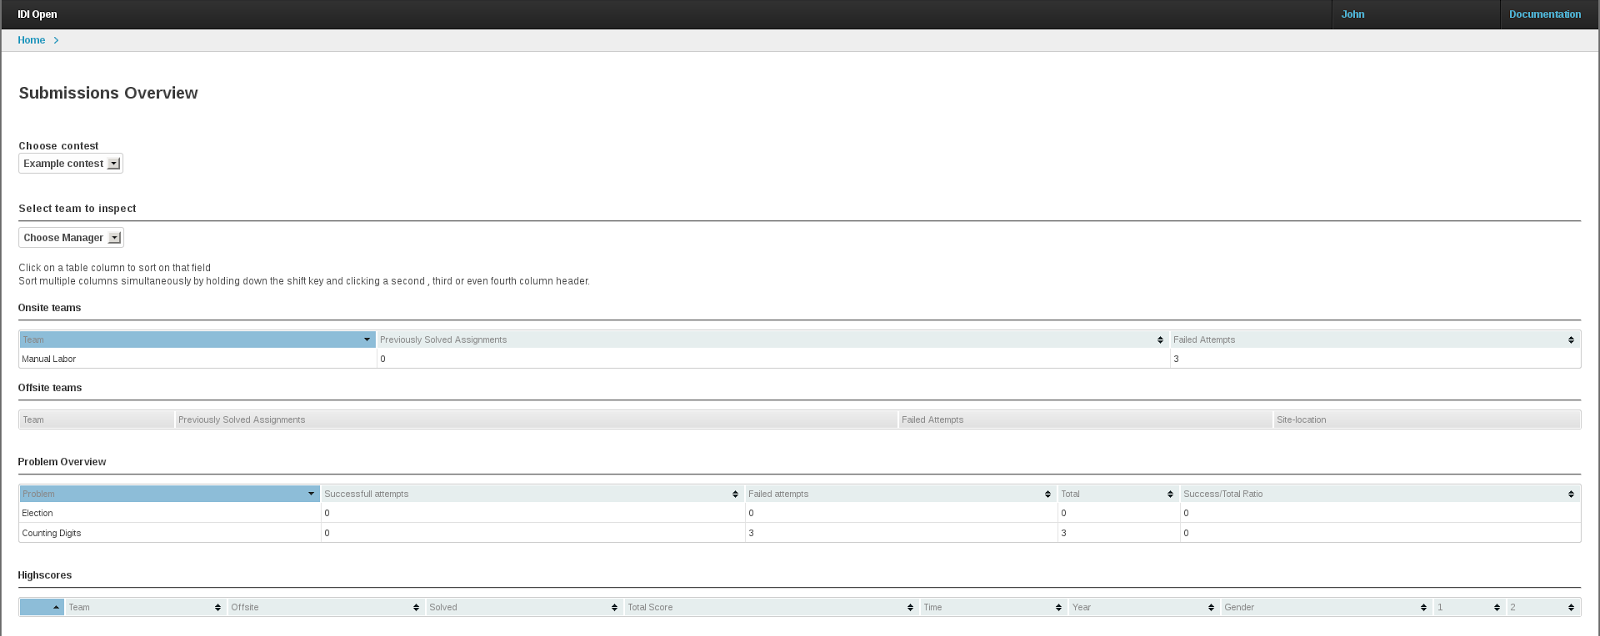
\includegraphics[width=0.8\textwidth]{Usermanual-img17.png}}
	\caption{Judge view}
	\label{fig:judgeView}
\end{figure}

\bigskip

Next up is two tables, one listing teams that are said to be onsite, the
other listing offsite teams. Other than the team names, there are two
columns in these tables, {\textquotedblleft}Previously solved
problems{\textquotedblright}, and {\textquotedblleft}Failed
attempts{\textquotedblright}. You can sort the table by clicking the
table header you want to sort by. This enables you to easily find the
teams that are struggling the most, sort the lists by the
{\textquotedblleft}Failed attempts{\textquotedblright} column. Clicking
the entries in these columns serve the same purpose as selecting a team
from the dropdown menu mentioned previously. 


\bigskip

Another table is present below the team tables. This is a table of the
problems in the system. The columns in this table are
{\textquotedblleft}Problem{\textquotedblright},
{\textquotedblleft}Successful attempts{\textquotedblright},
{\textquotedblleft}Failed attempts{\textquotedblright},
{\textquotedblleft}Total{\textquotedblright}, and
{\textquotedblleft}Success/Total ratio{\textquotedblright}. The
{\textquotedblleft}Problem{\textquotedblright} column states the names
of the given problem, {\textquotedblleft}Successful
attempts{\textquotedblright} is the number of submission that actually
solve the problem, and {\textquotedblleft}Failed
attempts{\textquotedblright} is the opposite.
{\textquotedblleft}Total{\textquotedblright} is the total number of
attempts at solving the problem that has been submitted to the system.
{\textquotedblleft}Success/Total ratio{\textquotedblright} is the ratio
of successful submissions for the given problem. As with the other
tables, this one can be sorted by any column. 


\bigskip

At the bottom of the site there is a highscore list. 


\bigskip

Finally, it{\textquoteright}s time to take a closer look at how you
should appropriately inspect a team{\textquoteright}s submissions.
Select the team in the drop down menu, or by clicking it in the list of
teams. Doing so will take you to the following site. 

\begin{figure}
\centering
	\frame{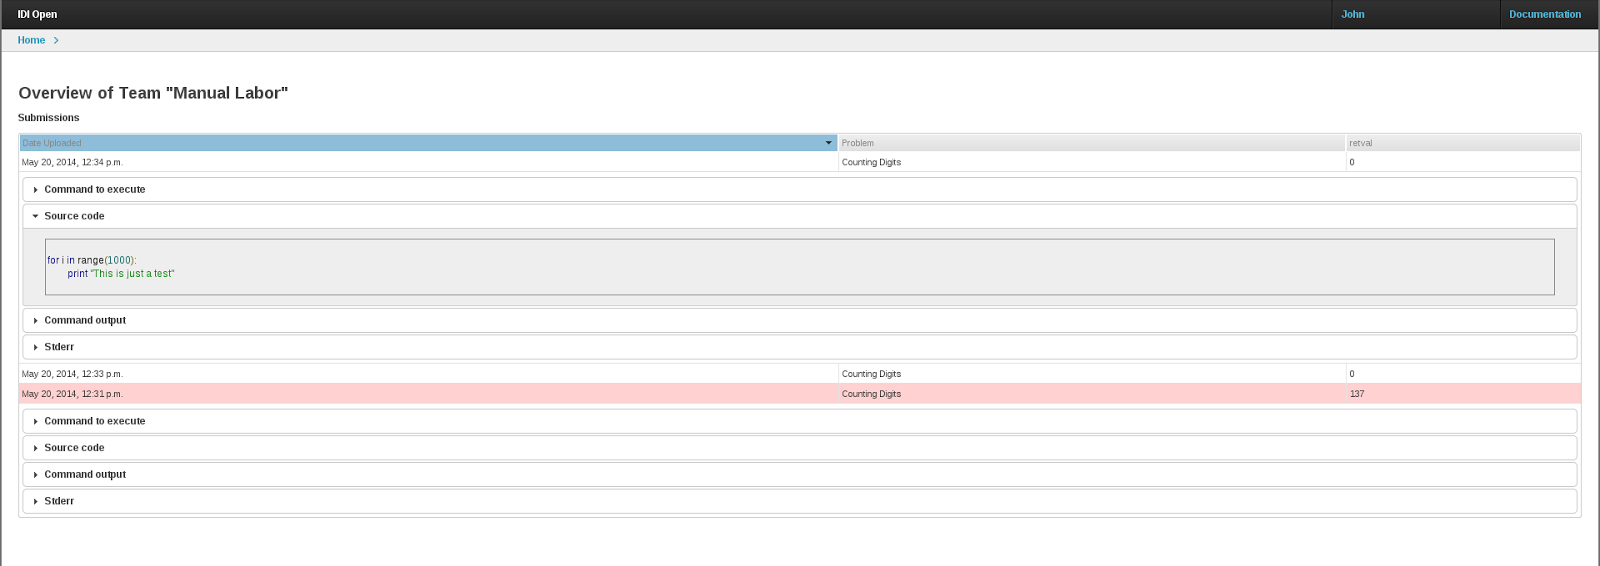
\includegraphics[width=0.8\textwidth]{Usermanual-img18.png}}
	\caption{Judge view for a team}
	\label{fig:judgeViewTeam}
\end{figure}

\bigskip

Initially you will see a simple table listing the submissions submitted
by the specified team. The columns are the following:
{\textquotedblleft}Date uploaded{\textquotedblright},
{\textquotedblleft}Problem{\textquotedblright}, and
{\textquotedblleft}retval{\textquotedblright}. The
{\textquotedblleft}Date uploaded{\textquotedblright} column lists the
date AND time that the submission was uploaded.
{\textquotedblleft}Problem{\textquotedblright} is simply which problem
the team intended their submission to solve. The column in need of
further explanation is {\textquotedblleft}retval{\textquotedblright},
this is the exit code of the submission execution, if this value is
nonzero an error of some sort has occurred. 


\bigskip

However, this is more than a simple listing. By clicking a row you
expand it, revealing four buttons, {\textquotedblleft}Command
executed{\textquotedblright}, {\textquotedblleft}Source
code{\textquotedblright}, {\textquotedblleft}Command
output{\textquotedblright}, and
{\textquotedblleft}Stderr{\textquotedblright}. By clicking these the
row will expand further and reveal more information. 


\bigskip

{\textquotedblleft}Command issued{\textquotedblright} is the command
that the system issued to execute the submission, e.g.
{\textquotedblleft}java Classname{\textquotedblright} for java programs
etc. {\textquotedblleft}Source code{\textquotedblright} is the source
code submitted by the team. {\textquotedblleft}Command
output{\textquotedblright} is the output produced by the execution of
the submitted source code.
{\textquotedblleft}Stderr{\textquotedblright} is the error messages
printed during execution. It is worth taking note of the fact that the
program used for measuring submission execution time will print the
time to stderr, this line will look something like
{\textquotedblleft}0.02{\textbackslash}n0.12{\textquotedblright} and
can be found at the bottom of the
{\textquotedblleft}Stderr{\textquotedblright}. 


\section{Contestant}

The users competing in the competition are considered contestants. In
this part of the guide we assume that appropriate links have been added
to the sidebar by admins. The only links that are in the sidebar by
default are the ones for registering a user and registering a team.

\subsection{Register User}

\begin{figure}
\centering
	\frame{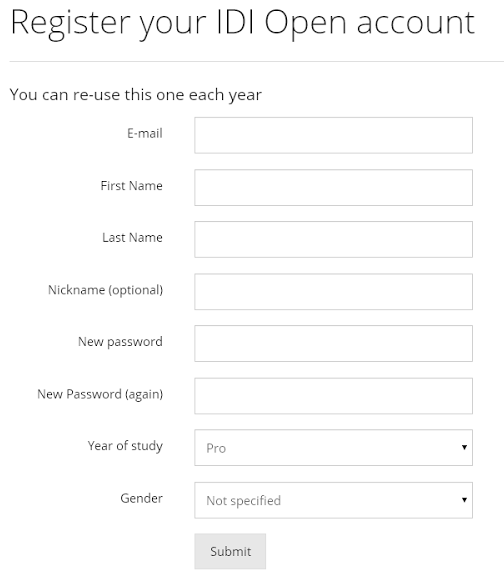
\includegraphics[width=0.8\textwidth]{Usermanual-img19.png}} 
	\caption{User registration}
	\label{fig:userReg}
\end{figure}

For user{\textquoteright}s who are not logged in there will always be a
{\textquotedblleft}Register user{\textquotedblright} button in the
sidebar. This button will take you to a form for submitting user
information. All of the fields are required, except for the nickname,
which is optional. The email field is used to send out user activation
emails and as such it is crucial that the email address is correct. The
{\textquotedblleft}Year of study{\textquotedblright} dropdown list
contains 6 different options, the integers from 1 to 5, and
{\textquotedblleft}Pro{\textquotedblright}. Students are to select the
integer corresponding to how far they{\textquoteright}ve come in their
study program, working professionals are to select the
{\textquotedblleft}Pro{\textquotedblright} option. The final option is
gender, which can be left as
{\textquotedblleft}Unspecified{\textquotedblright}, or set to male or
female.


\subsection{Edit User}

\begin{figure}
\centering
	\frame{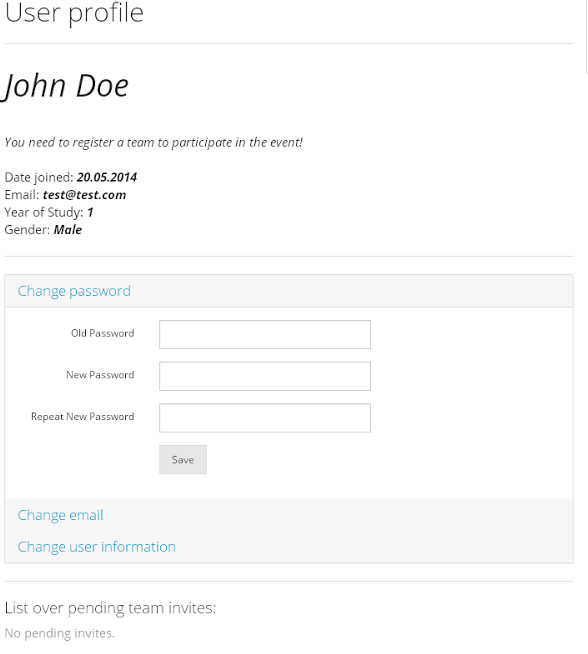
\includegraphics[width=0.8\textwidth]{Usermanual-img20.png}} 
	\caption{Edit user}
	\label{fig:editUser}
\end{figure}

On your user profile there are three buttons for editing your user,
{\textquotedblleft}Change email{\textquotedblright},
{\textquotedblleft}Change password{\textquotedblright}, and
{\textquotedblleft}Change user information{\textquotedblright}. The two
first are self-explanatory, they enable you to change your email and
password, in other words your login information. The
{\textquotedblleft}Change user information{\textquotedblright} option
lets you edit the rest of the fields you submitted during the
registration process, first name, last name, nickname, year of study,
and gender. It is worth noting that changing your email will send a new
activation email to the newly registered email address, if the new
address has not been activated within a given time limit the change
will not occur.

\subsection{Create Team}

If you{\textquoteright}ve got an account, but you{\textquoteright}re not
member of any team, there will be a link available to you in the
sidebar labeled {\textquotedblleft}Register team{\textquotedblright}.
This button will take you to a form for registering new teams. 

\begin{figure}
\centering
 \frame{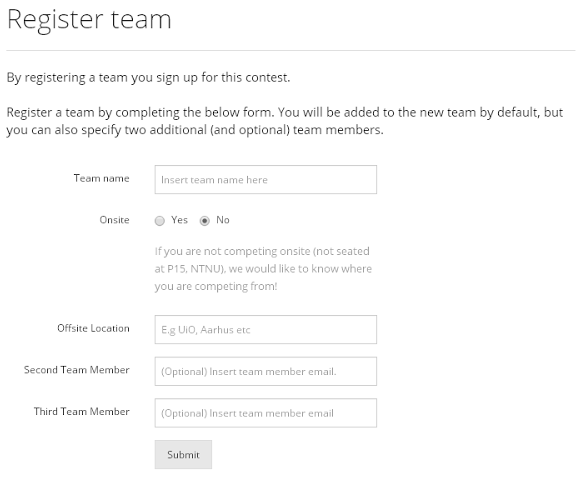
\includegraphics[width=0.8\textwidth]{Usermanual-img21.png}} 
 \caption{Create team}
 \label{fig:createTeam}
\end{figure}

The form requires that you give your team a name, and that you give some
information as to your location during the event. If you are planning
on being on-site during the contest all you need to do is select the
{\textquotedblleft}yes{\textquotedblright} radio button labeled onsite.
If you are not planning on being on-site, you need to fill out the
field labeled {\textquotedblleft}Offsite location{\textquotedblright}
with the location you are intended to stay in during the contest. 


In addition to this basic information you can invite team members while
you are at it. Just type in the email address of your to-be team
members in the fields {\textquotedblleft}Second Team
Member{\textquotedblright} and {\textquotedblleft}Third Team
Member{\textquotedblright}. They don{\textquoteright}t have to be
registered user{\textquoteright}s in the system to get the invite, they
will be notified of your invitation and will be able to accept the
invite upon registering their account. 

\subsection{Edit Team}

\subsubsection{Edit Basic Information}

On the team profile page there is a button labeled
{\textquotedblleft}Edit team{\textquotedblright}, if you press this
button it will take you to a form for editing your team. You need to be
the team leader for this option to be available to you. 

\begin{figure}
\centering
	\frame{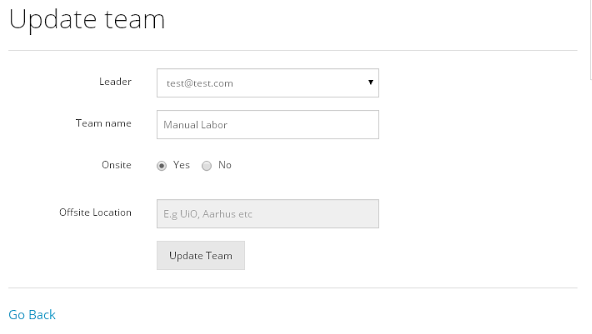
\includegraphics[width=0.8\textwidth]{Usermanual-img22.png}} 
	\caption{Edit team information}
	\label{fig:editTeamInfo}
\end{figure}

As with the editing of your user account, the same fields that were
available to you during registration of your team, are also available
when editing it. You can change your team name, and location. When you
are done making changes just click the {\textquotedblleft}Update
team{\textquotedblright} button and your changes will be put into
effect. 

Since the majority of team management is up to the team leader alone,
one might want to transfer the role of being team leader to another
team member. This can be done by selecting another team member in the
dropdown menu labeled {\textquotedblleft}Leader{\textquotedblright}.


\bigskip


\bigskip

\subsubsection{Invite User to Team/Join Team}

If you for some reason did not know who were to be on your team when you
created your team you can add them later on, given that you are the
team leader. This is done on your team profile page, the link is found
in the sidebar.

\begin{figure}
\centering
 \frame{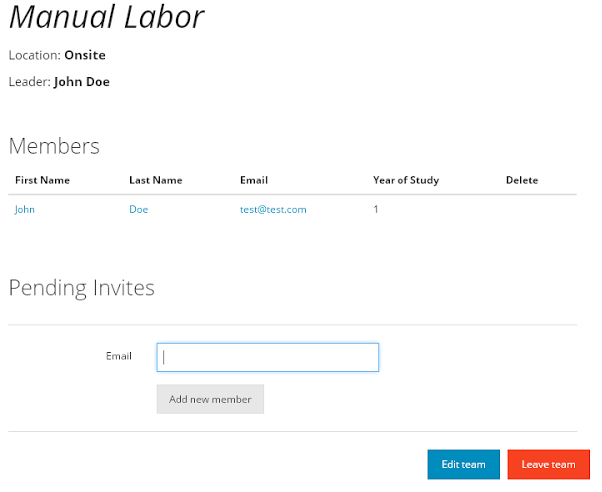
\includegraphics[width=0.8\textwidth]{Usermanual-img23.png}} 
 \caption{Invite team members}
 \label{fig:teamInvite}
\end{figure}

Inviting a member is done by writing their email address in the
{\textquotedblleft}Email{\textquotedblright} field and pressing the
{\textquotedblleft}Add new member{\textquotedblright} button. As
mentioned in the Create team section, your team members
don{\textquoteright}t need to be registered user{\textquoteright}s at
the time of you inviting them. They will be notified, and the invite
will be stored in the system and accessible to them when they finally
decide to create a user. 

\subsubsection{Remove User from Team}

\begin{figure}
\centering
 \frame{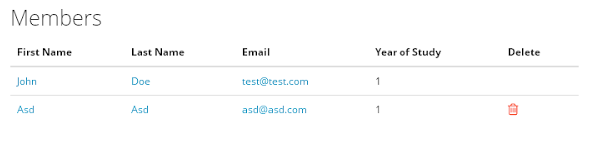
\includegraphics[width=0.8\textwidth]{Usermanual-img24.png}} 
 \caption{Remove user from team}
 \label{fig:teamRemoveUser}
\end{figure}

If you for some reason decide to evict a team member this can also be
done on your team profile page. The team profile lists all the team
members, to evict one, simply click the trashcan on the
user{\textquoteright}s entry. All user{\textquoteright}s can decide to
leave a team as they please, however, to evict other users in this
manner you need to be the team leader.


\bigskip

\subsection{Solve Problems}

Assuming your team is setup and the contest has started,
it{\textquoteright}s time to start actually competing. You get points
for solving problems, in other words, submitting source code that gives
correct output given the correct input.


To find the list of the problems in the contest problem set, just click
the {\textquotedblleft}Contest page{\textquotedblright} button in the
sidebar. This will take you to a page looking like the one in the
figure below.


\begin{figure}
\centering
 \frame{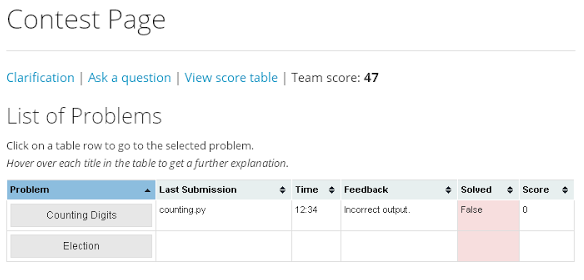
\includegraphics[width=0.8\textwidth]{Usermanual-img25.png}}  
 \caption{Problem overview}
 \label{fig:problemOverview}
\end{figure}

The contest that was used for creating this figure contained two
problems, Counting Digits, and Election. You can see that the user
logged in has already made an attempt at solving Counting Digits,
however it failed due to incorrect output. 


\bigskip

By clicking one of the rows you are taken to the site where you can
submit source code in an attempt at solving problems. 

\begin{figure}
\centering
 \frame{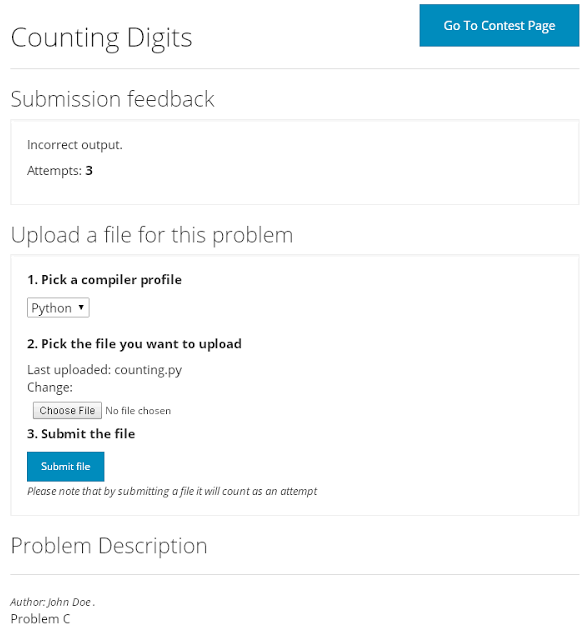
\includegraphics[width=0.8\textwidth]{Usermanual-img26.png}} 
 \caption{Submit problems}
 \label{fig:submitProblem}
\end{figure}

When submitting source code you need to specify what compiler profile is
suitable for the source you are submitting. If you{\textquoteright}re
submitting python code, select
{\textquotedblleft}python{\textquotedblright} in the dropdown menu
labeled {\textquotedblleft}1. Pick a compiler
profile{\textquotedblright}. Then upload your source by clicking the
{\textquotedblleft}Choose file{\textquotedblright} button, and then
press the {\textquotedblleft}Submit File{\textquotedblright} button.
Your source will then be submitted and evaluated. The site will
automatically update upon the evaluation of your submission being
completed. \ 

\subsection{Clarification}

During a contest contestants might need help understanding a certain
part of the system or a problem description. In order for them not
having to wander around looking for a functionary, they can post
questions that can be answered by the staff users. 

\subsubsection{Post a Question}

There is a link in the sidebar taking you to the site where you can post
questions. 

\begin{figure}
\centering
 \frame{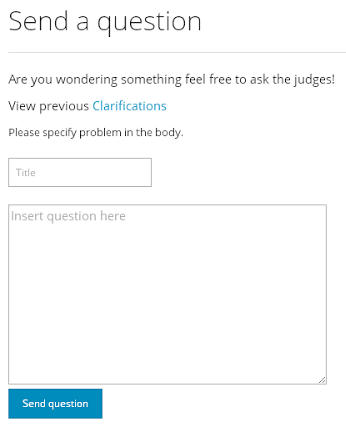
\includegraphics[width=0.8\textwidth]{Usermanual-img27.png}} 
 \caption{Post a question}
 \label{fig:clarificationQuestion}
\end{figure}

Posting a question is quite straight forward. Enter a title for your
question in the title field, and put the body of your question in the
largest textbox. When you are done writing and ready to post it, press
the {\textquotedblleft}Send question{\textquotedblright} button. Now
the question can be read and answered by the staff users. 

\subsubsection{Review Replies}

Questions posted through the clarification system are not visible for
anyone except the staff users, that is, unless they have been answered
by the staff. When a question has been answered it is visible to all
contestants.


\bigskip

As usual the link taking you to the list of answered questions can be
found in the sidebar. 

\begin{figure}
\centering
 \frame{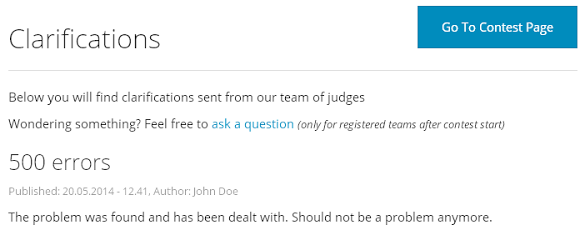
\includegraphics[width=0.8\textwidth]{Usermanual-img28.png}} 
 \caption{Clarification response}
 \label{fig:clarificationResponse}
\end{figure}

Here you can see that a staff user has answered the question posted. 



\subsection{Highscore List}

\subsubsection{Top Five}

On just about every part of the site there is a small highscore list
visible at the top right corner of the screen. This is simply a list of
the five teams with the best score. 

\subsubsection{Full Highscore}

The complete highscore list can be found by clicking the link labeled
{\textquotedblleft}All{\textquotedblright} in the top five high score
list, or by clicking the link labeled
{\textquotedblleft}Highscore{\textquotedblright} in the sidebar. This
is not just a list but a table which can be sorted by different
columns.
\begin{figure}
\centering
	\frame{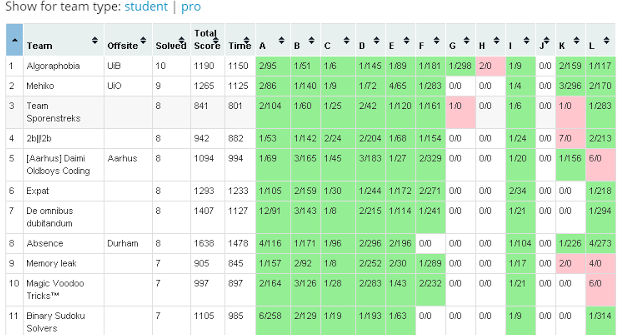
\includegraphics[width=0.8\textwidth]{Usermanual-img29.png}} 
	\caption{Full highscore}
	\label{fig:fullHighscore}
\end{figure}

The buttons labeled {\textquotedblleft}student{\textquotedblright} and
{\textquotedblleft}pro{\textquotedblright} lets you filter the
highscore. If you press the
{\textquotedblleft}student{\textquotedblright} button, all teams
containing professional members will be removed from the list. The
{\textquotedblleft}pro{\textquotedblright} button does the opposite. To
sort the table by a specific column, click the column label, to reverse
the ordering, click it again. The columns labeled by single characters
correspond to different problems. 

